\documentclass[11pt,english,a4paper,hidelinks]{book}
% settings.tex — LaTeX preamble configuration for TFG paper in English

\usepackage[utf8]{inputenc}      % Encoding
\usepackage[T1]{fontenc}         % Font encoding
\usepackage{mathpazo}            % Cursive text support
\usepackage[english]{babel}      % Language support
\usepackage[a4paper, margin=2.5cm]{geometry}  % Page size and margins
\usepackage{setspace}            % Line spacing
\usepackage{graphicx}            % Include images
\usepackage{amsmath, amssymb}    % Math packages
\usepackage{float}               % Improved float control
\usepackage{booktabs}            % Professional tables
\usepackage{hyperref}            % Hyperlinks in TOC, etc.
\usepackage{color, xcolor}       % Colors
\usepackage{lscape}              % Landscape pages
\usepackage{longtable}           % Tables spanning multiple pages
\usepackage{fancyhdr}            % Header/footer customization
\usepackage{titlesec}            % titulo formatting
\usepackage{caption}             % Caption formatting
\usepackage{biblatex}            % Bibliography handling
\usepackage{csquotes}            % Required by biblatex
\usepackage{tikz}                % For the cover page
\usepackage{ifthen}              % For the cover page
\usepackage{listings}            % For code listings
\usepackage{xcolor}              % For syntax highlighting

% Configure listings for Python-like VSCode white theme
\lstset{
    basicstyle=\ttfamily\small\color{black},
    keywordstyle=\color{blue!70!black},
    commentstyle=\color{green!50!black},
    stringstyle=\color{red!70!black},
    numberstyle=\color{gray!60},
    numbers=left,
    numbersep=2pt,
    frame=single,
    framerule=0.4pt,
    rulecolor=\color{gray!40},
    breaklines=true,
    breakatwhitespace=false,
    showstringspaces=false,
    tabsize=4,
    backgroundcolor=\color{gray!5},
    xleftmargin=10pt,
    xrightmargin=10pt,
    framexleftmargin=10pt,
    framexrightmargin=10pt,
    linewidth=\textwidth,
    captionpos=b,
    aboveskip=10pt,
    belowskip=10pt,
    literate={_}{\_}1
}

% Load bibliography file
\addbibresource{bibliography.bib}

% Section color
\definecolor{azul}{rgb}{0.1,0.2,0.4}

% Header/Footer styling
\pagestyle{fancy}
\fancyhf{}
\fancyhead[LE,RO]{\thepage}
\fancyhead[LO]{\leftmark}
\fancyhead[RE]{\rightmark}
\renewcommand{\headrulewidth}{0.4pt}
\renewcommand{\headrule}{\hbox to\headwidth{\color{azul}\leaders\hrule height \headrulewidth\hfill}}
\setlength{\headheight}{23.11996pt}
\newcommand{\arialbold}{\fontfamily{phv}\fontseries{b}\selectfont}

% Captions
\captionsetup{labelfont=bf, font=small}

% Section styling
\titleformat{\section}
  {\color{azul}\normalfont\Large\bfseries}
  {\thesection}{1em}{}

\titleformat{\subsection}
  {\color{azul}\normalfont\large\bfseries}
  {\thesubsection}{1em}{}

% Metadata (centralized definitions)
\newcommand{\titulo}{Evaluating Score-Investing Methodologies:
A Systematic Review of Tweenvest's Algorithm for Long-Term Stock Investing Using Descriptive Analytics and Predictive Modeling.
}
\newcommand{\tutorA}{Joaquín Martínez Minaya (GADE)}
\newcommand{\tutorB}{Alberto Albiol Colmener (GITST)} 
\newcommand{\tutorC}{José Tatay Sangüesa (Tweenvest)} 
\newcommand{\curso}{2024-2025}
\newcommand{\autor}{Carlos Eduardo Domínguez Martínez}
\newcommand{\fecha}{June 2025}



% Add bibliography configuration
\addbibresource{bibliography.bib}

\begin{document}
\renewcommand{\listtablename}{List of Tables} 
\renewcommand{\tablename}{Table} 

% ############################### COVER PAGE #######################
\thispagestyle{empty}
\usetikzlibrary{calc}


\begin{tikzpicture}[overlay,remember picture]
\fill[fill=white] (current page.south west) rectangle ($(current page.south east)+(0,4cm)$);

% Logos at top
\node at ($(current page.north)+(-6.37cm,-1.8cm)$) 
  {\includegraphics[scale=0.495]{images/logos/TFG UPV Principal Negro.pdf}};
\node at ($(current page.north)+(6.7cm,-1.77cm)$) 
  {\includegraphics[trim=11.8cm 10.8cm 11.5cm 8.05cm,clip,width=0.233\textwidth]{images/logos/TFG Telecom VLC 2018.pdf}};

% titulo
\node[anchor=center] at ($(current page.center)!0.35!(current page.north)+(0cm,0)$) (titulo)
  {\begin{minipage}{1.05\textwidth}\begin{center}\Large\textbf{\uppercase{\titulo}}\end{center}\end{minipage}};

% Degree and university text block
\node[anchor=north west] at  ($(current page.center)+(-1.45cm,-5.6cm)$) (){\parbox{0.59\textwidth}{%
\tolerance=1%
\emergencystretch=\maxdimen%
\hyphenpenalty=10000%
\hbadness=10000%
\normalsize\rmfamily Trabajo Fin de Grado presentado en la Escuela Técnica 
Superior  de  Ingeniería  de  Telecomunicación  de  la 
Universitat  Politècnica  de  València, para  la  obtención 
del Doble Título de Graduado en Adiminstración y Dirección de Empresas e Ingeniería de Tecnologías y 
Servicios de Telecomunicación\\
\ \\
Curso \curso\\
\ \\
València, \fecha}};

% Tutors
\node[anchor=center] at ($(current page.center)+(0cm,-0.8cm)$) (tutor) {\bfseries Co-Tutor: \tutorA};
\node[anchor=center] at ($(current page.center)+(0cm,-1.55cm)$) {\bfseries \ifthenelse{\equal{\tutorB}{}}{}{Co-Tutor: \tutorB}};
\node[anchor=center] at ($(current page.center)+(0cm,-2.3cm)$) {\bfseries \ifthenelse{\equal{\tutorC}{}}{}{Co-Tutor: \tutorC}};

% Author (placed between titulo and tutor)
\node[coordinate] at ($(titulo.south)!(tutor.north)!(titulo.south)$) (tutornorte){};
\node at ($(titulo.south)!0.54!(tutornorte)$) 
  {\begin{minipage}{\textwidth}\begin{center}\large\textbf{\autor}\end{center}\end{minipage}};

% Contact info block at bottom left
\node[opacity=1,anchor=south west,scale=0.9] at ($(current page.south west)+(1.9,1.825)$)
  {\parbox{0.75\textwidth}{%
\scriptsize{\fontfamily{phv}\selectfont
Escuela Técnica Superior de Ingeniería de Telecomunicación\\[0.5mm]
Universitat Politècnica de València\\[0.5mm]
Edificio 4D. Camino de Vera, s/n, 46022 Valencia\\[0.5mm]
Tel. +34 96 387 71 90, ext. 77190\\[1.25mm]
\resizebox{3.15cm}{2.5mm}{\arialbold \href{http://www.etsit.upv.es}{www.etsit.upv.es}}}}};

% Extra logos at bottom right
\node[opacity=1,anchor=south east] at ($(current page.south east)+(-2,1.34)$)
  {
\includegraphics[scale=0.16]{images/logos/Extra Logos TFG.png}};

\end{tikzpicture}

\newpage
 
% ############################### ABSTRACT ###############################
\newpage
\thispagestyle{empty}\ \\
\newpage
\thispagestyle{empty}

\section*{Abstract}
\noindent This study investigates the effectiveness of a factor-investing methodology developed by Tweenvest, leveraging a proprietary algorithm grounded in fundamental financial analysis. The algorithm scores companies across four key factors: Quality, Growth, Value, and Dividends.

\vspace{0.5cm}

\noindent The research aims to evaluate the profitability of investment strategies based on these scores over multiple profitability horizons from 1 month to five years. A comprehensive dataset was constructed, integrating factor scores with additional variables such as sector and geographic region, standardized for currency and timeframes.

\vspace{0.5cm}

\noindent Statistical analyses will explore relationships between these factors and returns, identifying optimal investment periods. Subsequently, predictive modeling—including econometric regressions, time series models, and neural networks—will be applied to assess the translation of these factors into market performance.

\vspace{0.5cm}

\noindent The study incorporates an interdisciplinary approach, combining financial theory and econometrics with advanced programming, data engineering, and artificial intelligence. This integration bridges Business Management and Telecommunications Engineering, offering insights into the practical application of Tweenvest's scoring algorithm and contributing to the advancement of financial technology analytics.


% ############################### DEDICATION #######################
\newpage
\thispagestyle{empty}
\vfill
\begin{flushright}
To my parents.
\end{flushright}
\vfill\vfill

% ############################### TABLE OF CONTENTS #######################
\newpage
\thispagestyle{empty}
\ \\
\addtocontents{toc}{\protect\thispagestyle{empty}}
\addtocontents{toc}{\protect\pagestyle{empty}}
\tableofcontents
\newpage

% ############################### LIST OF FIGURES AND TABLES #######################
\addtocontents{lof}{\protect\thispagestyle{empty}}
\addtocontents{lof}{\protect\pagestyle{empty}}
\listoffigures
\newpage

\addtocontents{lot}{\protect\thispagestyle{empty}}
\addtocontents{lot}{\protect\pagestyle{empty}}
\listoftables
\newpage

% ############################### ACRONYMS / CAPITALIZED TERMS #######################
% Economic acronyms
\newacronym{soe}{SOE}{State-Owned Enterprise}
\newacronym{marketcap}{Market Cap}{Market Capitalization}

% Financial ratios acronyms
\newacronym{roa}{ROA}{Return on Assets}
\newacronym{roe}{ROE}{Return on Equity}
\newacronym{roic}{ROIC}{Return on Invested Capital}
\newacronym{roce}{ROCE}{Return on Capital Employed}
\newacronym{croic}{CROIC}{Cash Return on Invested Capital}
\newacronym{croce}{CROCE}{Cash Return on Capital Employed}
\newacronym{fcf}{FCF}{Free Cash Flow}

\newacronym{ebit}{EBIT}{Earnings Before Interest and Taxes}
\newacronym{ebitda}{EBITDA}{Earnings Before Interest, Taxes, Depreciation, and Amortization}

\newacronym{financialleverage}{Financial Leverage}{\ensuremath{\frac{\text{Total Assets}}{\text{Total Equity}}}}

\newacronym{currentratio}{Current Ratio}{\ensuremath{\frac{\text{Current Assets}}{\text{Current Liabilities}}}}
\newacronym{quickratio}{Quick Ratio}{\ensuremath{\frac{\text{Current Assets} - \text{Inventory}}{\text{Current Liabilities}}}}
\newacronym{cashratio}{Cash Ratio}{\ensuremath{\frac{\text{Cash and Equivalents}}{\text{Current Liabilities}}}}
\newacronym{ocfratio}{OCF Ratio}{\ensuremath{\frac{\text{Operating Cash Flow}}{\text{Current Liabilities}}}}

\newacronym{dps}{DPS}{Dividends per Share}
\newacronym{eps}{EPS}{Earnings per Share}
\newacronym{capex}{CAPEX}{Capital Expenditures}
\newacronym{cagr}{CAGR}{Compound Annual Growth Rate (\ensuremath{\left(\frac{\text{Ending Value}}{\text{Beginning Value}}\right)^{\frac{1}{n}} - 1})}

\newacronym{pe}{P/E}{\ensuremath{\frac{\text{Market Cap}}{\text{Adjusted TTM Earnings}}}}
\newacronym{ps}{P/S}{\ensuremath{\frac{\text{Market Cap}}{\text{TTM Revenue}}}}
\newacronym{pcf}{P/CF}{\ensuremath{\frac{\text{Market Cap}}{\text{TTM Operating Cash Flow}}}}
\newacronym{pb}{P/B}{\ensuremath{\frac{\text{Market Cap}}{\text{Tangible Equity}}}}

\newacronym{ttm}{TTM}{Trailing Twelve Months}

\newacronym{evsales}{EV/Sales}{\ensuremath{\frac{\text{Enterprise Value}}{\text{TTM Revenue}}}}
\newacronym{evebitda}{EV/EBITDA}{\ensuremath{\frac{\text{Enterprise Value}}{\text{TTM EBITDA}}}}
\newacronym{evebit}{EV/EBIT}{\ensuremath{\frac{\text{Enterprise Value}}{\text{TTM EBIT}}}}
\newacronym{evfcf}{EV/FCF}{\ensuremath{\frac{\text{Enterprise Value}}{\text{TTM Free Cash Flow}}}}

\newacronym{dividendyield}{Dividend Yield}{\ensuremath{\frac{\text{Dividend per Share}}{\text{Price per Share}} \times 100\%}}

% Math definitions for payout and dividend ratios
\newacronym{payoutratioeps}{Payout Ratio EPS}{\ensuremath{\frac{\text{DPS}}{\text{EPS}}}}
\newacronym{payoutratiofcf}{Payout Ratio FCF}{\ensuremath{\frac{\text{DPS}}{\text{FCF}}}}
\newacronym{payoutratioowner}{Payout Ratio Owner Earnings}{\ensuremath{\frac{\text{DPS}}{\text{Owner}}}}



% Technical/Code acronyms
\newacronym{ci/cd}{CI/CD}{Continuous Integration/Continuous Deployment}
\newacronym{ocr}{OCR}{Optical Character Recognition}
\newacronym{pairplot}{Pair Plot}{Pairwise relationship plot}
\newacronym{db}{DB}{Database}
\newacronym{job}{Job}{Code script that is executed by the system to perform a task, this could be a daily update of the financial information of the stocks, or a necessary action such as sending emails to get authentication pins.}
\newacronym{cron}{Cron}{Cron is a time-based job scheduler in Unix-like computer operating systems. It is used to schedule jobs (commands or shell scripts) to run at specified time intervals. Cron is typically used to automate tasks that need to be performed on a regular basis, such as backups, system maintenance, or data processing.}
\newacronym{unittest}{Unit Test}{Unit test is a type of software testing where individual units or components of a software are tested. The purpose of unit testing is to validate that each unit of the software performs as expected. Unit tests are typically written by the developers and run automatically as part of the development process.}
\newacronym{redis}{REDIS}{REDIS is an open-source, in-memory data structure store, used as a database, cache, and message broker. It supports data structures such as strings, hashes, lists, sets, and sorted sets with range queries, transactions, and different levels of on-disk persistence.}
\newacronym{args}{Args}{Arguments or inputs of a function}
\newacronym{decorator}{Decorator}{Decorator is a function that takes another function and extends the behavior of the original function without explicitly modifying it. Decorators are typically used to add functionality to functions, such as logging, caching, or authentication.}

\newacronym{iqr}{IQR}{Interquartile Range}
\newacronym{svm}{SVM}{Single Vector Machine}
\newacronym{if}{IF}{Isolation Forest}
\newacronym{lof}{LOF}{Local Outlier Factor}
\newacronym{multi}{MCOD}{Multi-Criteria Outlier Detection}
\newacronym{mcod}{MCOD}{Multi-Criteria Outlier Detection}
\newacronym{islandcase}{ICD}{Island Cases Detection}

\newacronym{gam}{GAM}{Generalized Additive Model}
\newacronym{nn}{NN}{Neural Network}
\newacronym{shap}{SHAP}{SHapley Additive exPlanations}
\newacronym{arima}{ARIMA}{AutoRegressive Integrated Moving Average}

\newacronym{rmse}{RMSE}{Root Mean Square Error}
\newacronym{mae}{MAE}{Mean Absolute Error}
\newacronym{r2}{R^2}{R-squared}


% ############################### START OF CONTENT #######################
\clearpage
\pagenumbering{arabic}
\setcounter{page}{1}
\addtocontents{toc}{\protect\thispagestyle{empty}}

\part{Main Report}

% ############################### INTRODUCTION #######################
\chapter{Introduction to Fundamental Analysis}
\section{Definition}

\noindent Fundamental Analysis is a methodology used to evaluate the intrinsic value of a company, asset, or market by analyzing various economic, financial, and qualitative and quantitative factors. Unlike technical analysis, which focuses on price movements and chart patterns, fundamental analysis seeks to determine an asset’s “true value” to identify investment opportunities that may be undervalued or overvalued in the market.
\vspace{0.5cm}

\noindent This intrinsic value is defined by numerous experts and renowned investors, including Benjamin Graham, Warren Buffett, and Pat Dorsey [II]; and many Stock’s Index such as IBEX-35 or MSCI, as a company’s ability to adapt to an ever-changing environment while adding value to the market and establishing barriers to entry for competitors—commonly known as economic moats.
\vspace{0.5cm}

\noindent Measuring these moats is challenging due to the difficulty of quantifying certain variables, such as brand strength and market influence. However, over the long term, these intangible factors translate into tangible financial data, reflected in a company’s balance sheet, income statement, and cash flow statement; that when exposed to the public market share creates a need to buy or sell the stocks, altering the companies profitability. So from now on, this economic moats will be called \textit{alpha}, following the common literature. 

\section{Tweenvest's Scores}
Following this approach, Tweenvest developed its four main scores based on key focus areas that investors have to consider before making any decision:
\begin{itemize}
    \item Profitability
    \item Financial Health
    \item Predictability
    \item Consistent Growth
    \item Entrance Moment
    \item Dividends Payed
\end{itemize}

\subsection{Quality}

\noindent This Tweenvest's score is approached in a similar way that many successful investors would, distinguishing on three main categories: \textbf{profitability}, \textbf{financial health}, and \textbf{predictability}. Each of them includes inside of them multiple financial ratios that take account of different relevant data within the company's reports.

\vspace{0.5cm}
\noindent To understand the complexity of this score, we need to look at each category separately. Starting with \textbf{profitability} we can separate:

\subsubsection{Profitability Margins}
These are essential for understanding how a company is managing its costs and generating profits from its revenues.
\begin{itemize}
    \item \textbf{Net margin}: Represents net profit as a percentage of total sales, indicates a company's efficiency in generating profits after accounting for all expenses, taxes, and costs. A high net margin suggests that the company has good cost control and strong pricing power in the market.
    
    \item \textbf{Operating margin}: Measures operating profit (EBIT) as a percentage of total sales, providing a clear view of the profitability of a company's core operations, excluding interest and taxes. This metric is fundamental for evaluating a company's operational efficiency.
    
    \item \textbf{EBITDA margin}: Removes the effects of capital structure and accounting policies, offering a clear view of the company's pure operational profitability.
    
    \item \textbf{Gross margin}: Focuses on revenues after deducting the cost of goods sold, is a key measure of production efficiency and a company's ability to manage its direct costs.
\end{itemize}

\subsubsection{Performance Ratios}
These are used to measure the overall performance of the company.
\begin{itemize}
    \item \textbf{ROA (Return on Assets)}: Measures how efficiently a company converts its assets into profits. This is especially important in capital-intensive sectors, where efficient asset management can make a significant difference in profitability.
    
    \item \textbf{ROE (Return on Equity)}: Focuses on the profits generated per dollar of equity invested by shareholders. This ratio is crucial for evaluating a company's overall profitability from the shareholders' perspective. It is an especially valuable metric for investors seeking to maximize their returns on equity investment.
    
    \item \textbf{ROIC (Return on Invested Capital)}: Focuses on the return generated by all the funds invested in the company, including both shareholders' equity and debt. It is a comprehensive measure of a company's ability to generate value from all its sources of financing.
    
    \item \textbf{ROCE (Return on Capital Employed)}: Measures the funds used to finance operations, regardless of the source. This ratio is useful for comparing the efficiency of companies with different capital structures, as it focuses on total capital employed rather than just equity.
\end{itemize}

\noindent Also, to not only look at actives Tweenvest uses the cash generated to calculate: \textbf{CROIC} (Cash Return on Invested Capital), \textbf{CROCE} (Cash Return on Capital Employed), \textbf{OCF/Sales}, and \textbf{FCF/Sales}. And lastly it takes account also the Owner's income to calculate: \textbf{Owner's Income/Sales}, \textbf{Owner's CROIC} and \textbf{Owner's CROCE}.

\vspace{0.5cm}
\noindent Continuing with the financial health, we need to analyze the company’s debt in multiple aspects:

\subsubsection{Leverage Ratios}
These ratios assess how much a company relies on debt to finance its assets and operations. They are essential for evaluating financial risk and long-term solvency.
\begin{itemize}
    \item \textbf{Financial Leverage} (Total Assets / Equity): Measures the proportion of a company's assets that are financed by shareholder equity. A higher ratio suggests the company is using more debt relative to equity, indicating greater financial risk but also potential return amplification through leverage.
    
    \item \textbf{Total Debt/Assets}: Indicates what portion of the company's assets is financed through debt. A lower ratio implies a more conservative capital structure, while a higher one may indicate increased risk if the company becomes over-leveraged.
    
    \item \textbf{Total Debt/Capital}: Measures the share of total capital (debt + equity) that comes from debt. This ratio is useful for understanding how dependent the company is on borrowed funds compared to its overall capital base.
    
    \item \textbf{Total Debt/Equity}: Compares the company's total debt to its shareholder equity. It provides insight into the balance between debt and equity financing. A high ratio may signal financial risk, but also the potential for higher returns if debt is managed well.
\end{itemize}

\subsubsection{Debt Coverage Ratios}
These metrics evaluate a company's ability to cover its debt using its earnings or cash flow. They reflect the sustainability of a company's debt in relation to its operational performance.

\begin{itemize}
    \item \textbf{Net Debt/EBIT}: Shows how many years it would take for a company to repay its net debt using EBIT (Earnings Before Interest and Taxes).
    
    \item \textbf{Net Debt/EBITDA}: Similar to the above, but adds back depreciation and amortization. This gives a more cash-focused view of a company's ability to handle its debt load, and is especially useful for comparing companies in capital-intensive industries.
    
    \item \textbf{Net Debt/FCF}: Evaluates how many years of free cash flow would be needed to pay off net debt. Since FCF includes investment needs, this ratio gives a more conservative view of debt sustainability.
    
    \item \textbf{Net Debt/Owner's Income}: Compares net debt to the income available to equity holders (after all operating and investing costs).
\end{itemize}

\subsubsection{Interest Coverage Ratios}
These ratios measure how easily a company can meet its interest payments on outstanding debt — critical for assessing short-term debt service capability.

\begin{itemize}
    \item \textbf{EBIT/Interest}: Indicates how many times a company can cover its interest expenses with its operating income.
    
    \item \textbf{EBITDA/Interest}: Similar to the above, but adds back depreciation and amortization. This gives a clearer picture of available cash earnings before fixed financial obligations, ideal for heavily asset-based businesses.
    
    \item \textbf{FCF/Interest}: Since FCF considers investment needs, this is a stringent test of how much real, discretionary cash is available for debt servicing.
    
    \item \textbf{Owner Earnings/Interest}: Evaluates a company's ability to meet interest payments based on the earnings effectively attributable to shareholders. It accounts for operational cash flow minus necessary capital expenditures.
\end{itemize}

\subsubsection{Liquidity Ratios}
These ratios measure a company's ability to meet short-term obligations with its short-term assets. They are essential for evaluating near-term financial health and risk of insolvency.

\begin{itemize}
    \item \textbf{Current Ratio} (Current Assets / Current Liabilities): Shows whether a company has enough assets to cover its short-term liabilities. A value above 1 is generally considered healthy, though excessively high values may imply inefficiency.
    
    \item \textbf{Quick Ratio} ((Current Assets - Inventory) / Current Liabilities): A more stringent version of the current ratio that excludes inventory, which may not be easily liquidated. It's useful in assessing true short-term liquidity.
    
    \item \textbf{Cash Ratio} (Cash and Equivalents / Current Liabilities): The most conservative liquidity metric, focusing only on cash and equivalents. It shows the immediate solvency of a company in a worst-case scenario.
    
    \item \textbf{OCF Ratio} (Operating Cash Flow / Current Liabilities): Assesses how well the company's operational cash flows can cover its current obligations. This offers a realistic view of liquidity since it's based on actual cash generation rather than accounting figures.
\end{itemize}

\subsubsection{Predictability}

\noindent And finally, for the quality score we need to look at the company’s predictability. This is achieved by trying to fit values related to the company’s success —such as Sales— to a exponential curve, which is supported by large financial literature.

\vspace{0.5cm}
\noindent After calculating all of this ratios, Tweenvest compares them to the sectors’ median and interpolates it to create a single score for each ratio and then aggregates them all using personalized weights to create the final Quality Score, which is then showed to the clients:

\begin{figure}[H]
    \centering
    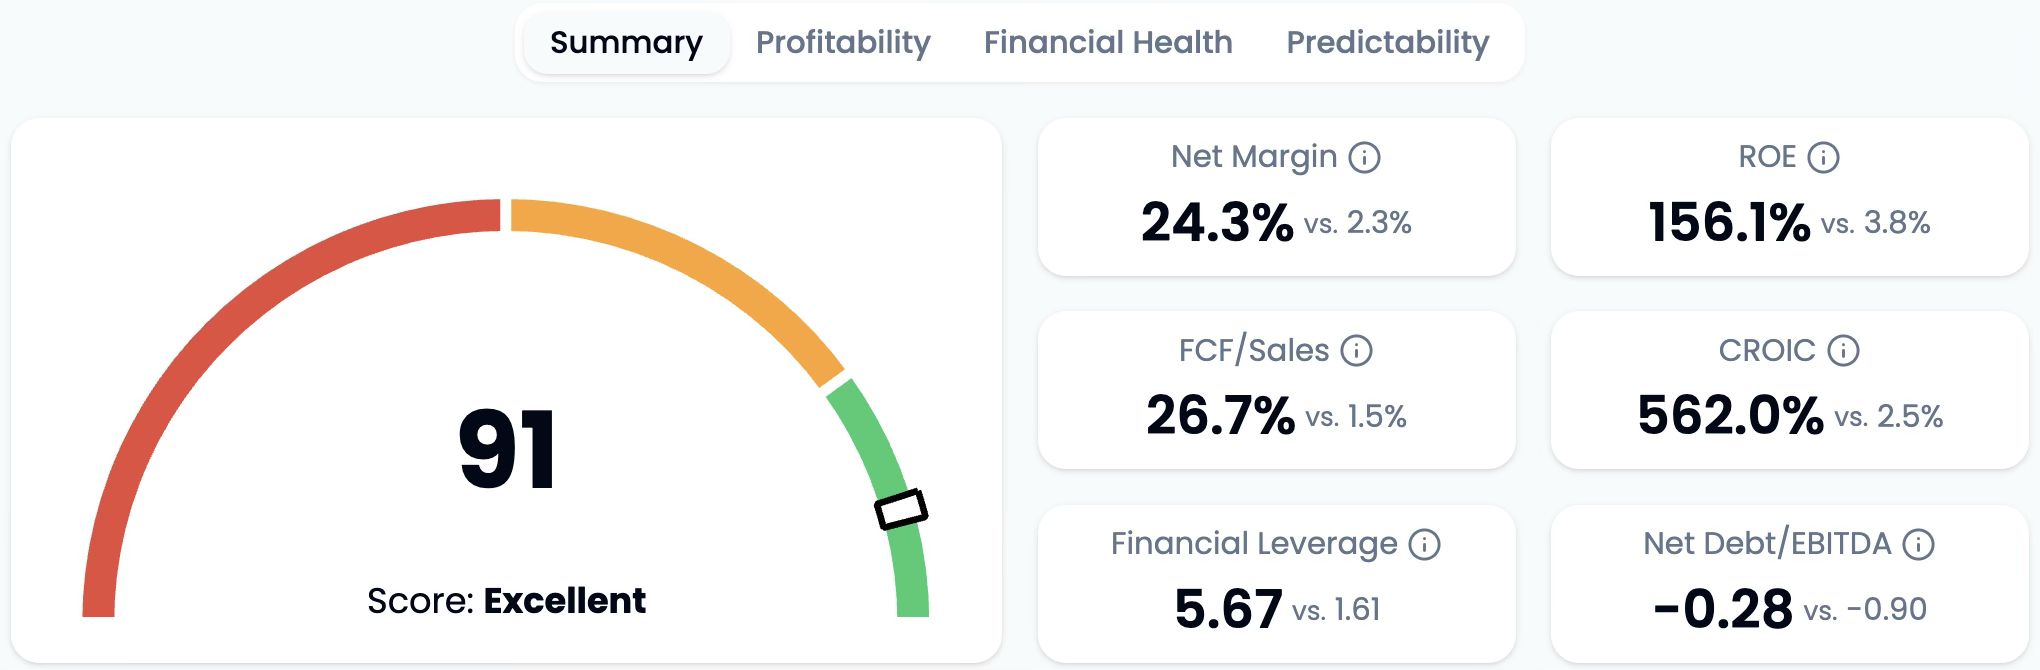
\includegraphics[width=0.8\textwidth]{images/tweenvest/quality score.png}
    \caption{Tweenvest's Quality Score}
    \label{fig:quality_score}
\end{figure}

\subsection{Growth}
\noindent The Growth Score evaluates a company's historical growth across multiple key metrics, comparing them to industry standards. This comprehensive approach ensures a balanced assessment of growth across different aspects of the business.

\subsubsection{Revenue \& Profitability Growth}
\begin{itemize}
    \item \textbf{Sales}: Measures growth in core revenue streams
    \item \textbf{EBITDA}: Captures growth in operational cash-generating ability before non-cash and financing impacts
    \item \textbf{Operating Income}: Reflects growth in profit from core business operations
    \item \textbf{Net Income}: Includes all income sources, showing overall profitability growth
\end{itemize}

\subsubsection{Cash Flow Growth}
\begin{itemize}
    \item \textbf{Operating Cash Flow}: Measures growth in cash generation from operations
    \item \textbf{Simple FCF}: A straightforward proxy for available cash after essential investments
    \item \textbf{Levered/Unlevered FCF}: Provide detailed views of free cash flow with and without debt impact
    \item \textbf{Owner Earnings}: Useful for volatile capex cases, emphasizing cash available to shareholders
\end{itemize}

\subsubsection{Capital Base Expansion}
\begin{itemize}
    \item \textbf{Total Assets}: Indicates expansion in overall asset base
    \item \textbf{Equity}: Reflects growth in shareholders' claim on the business
    \item \textbf{Tangible Book Value}: Highlights growth in physical net assets, excluding intangibles
    \item \textbf{Invested Capital}: Captures total capital being put to productive use
    \item \textbf{Capital Employed}: A broader measure of capital supporting business operations
\end{itemize}

\subsubsection{Per-Share Value Growth}
\begin{itemize}
    \item \textbf{Diluted EPS}: Tracks per-share earnings growth, accounting for dilution effects
    \item \textbf{Diluted Shares}: Included to track share count changes, ensuring EPS growth isn't artificially inflated by buybacks or dilution
    \item \textbf{Ordinary DPS}: Tracks the growth of shareholder payouts, a proxy for confidence in future earnings
\end{itemize}

\vspace{0.5cm}
\noindent To compute the Growth Score, Tweenvest calculates 10-year, 5-year, and 3-year averages and then interpolates the growth rate to industry standards. This approach reinforces the long-term investment philosophy, giving lasting growing companies a better score.

\begin{figure}[H]
    \centering
    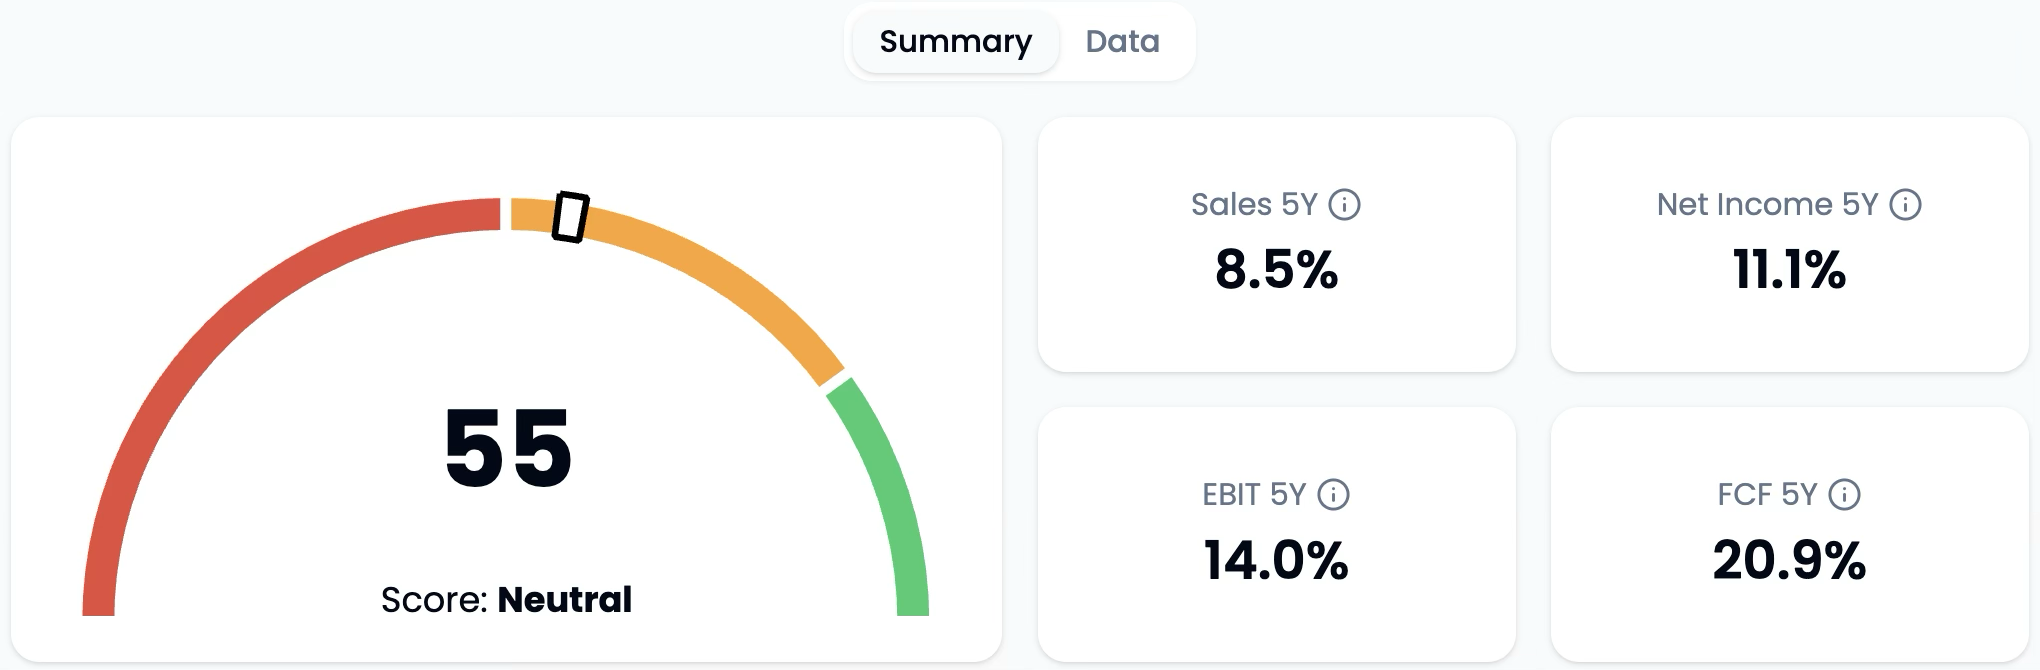
\includegraphics[width=0.8\textwidth]{images/tweenvest/growth score.png}
    \caption{Tweenvest's Growth Score}
    \label{fig:growth_score}
\end{figure}

\subsection{Valuation}
\noindent The Valuation Score measures how attractively a company is priced relative to its fundamentals such as earnings, cash flow, sales, and dividends. This is critical for investors following value investing principles, where the goal is to buy quality companies for less than their intrinsic worth. The algorithm evaluates a series of valuation multiples—both price-based and enterprise value-based—and dividend yield.

\subsubsection{Price-Based Multiples}
\begin{itemize}
    \item \textbf{P/E} (Market Cap / Adjusted TTM Earnings): Measures how much investors are willing to pay per dollar of earnings
    \item \textbf{P/S} (Market Cap / TTM Revenue): Useful when earnings are volatile; shows valuation relative to sales
    \item \textbf{P/CF} (Market Cap / TTM Operating Cash Flow): Reflects valuation relative to cash-generating ability
    \item \textbf{P/B} (Market Cap / Tangible Equity): Especially relevant for asset-heavy sectors like banks or industrials
\end{itemize}

\subsubsection{Enterprise Value-Based Multiples}
\begin{itemize}
    \item \textbf{EV/Sales} (Enterprise Value / TTM Revenue)
    \item \textbf{EV/EBITDA} (Enterprise Value / TTM EBITDA)
    \item \textbf{EV/EBIT} (Enterprise Value / TTM EBIT)
    \item \textbf{EV/FCF} (Enterprise Value / TTM Free Cash Flow)
\end{itemize}

\subsubsection{Yield-Based Valuation}
\begin{itemize}
    \item \textbf{Dividend Yield (\%)} (Dividend per Share / Price per Share)
\end{itemize}

\vspace{0.5cm}
\noindent Each of these ratios is compared to multiple historical statistics and sectoral benchmarks to create individual scores and then average them.

\vspace{0.5cm}
\noindent \textbf{Note:}
\begin{itemize}
    \item Market Cap = Share Price × Total Outstanding Shares
    \item Enterprise Value = Market Capitalization + Total Debt - Cash + Marketable Securities
\end{itemize}

\begin{figure}[H]
    \centering
    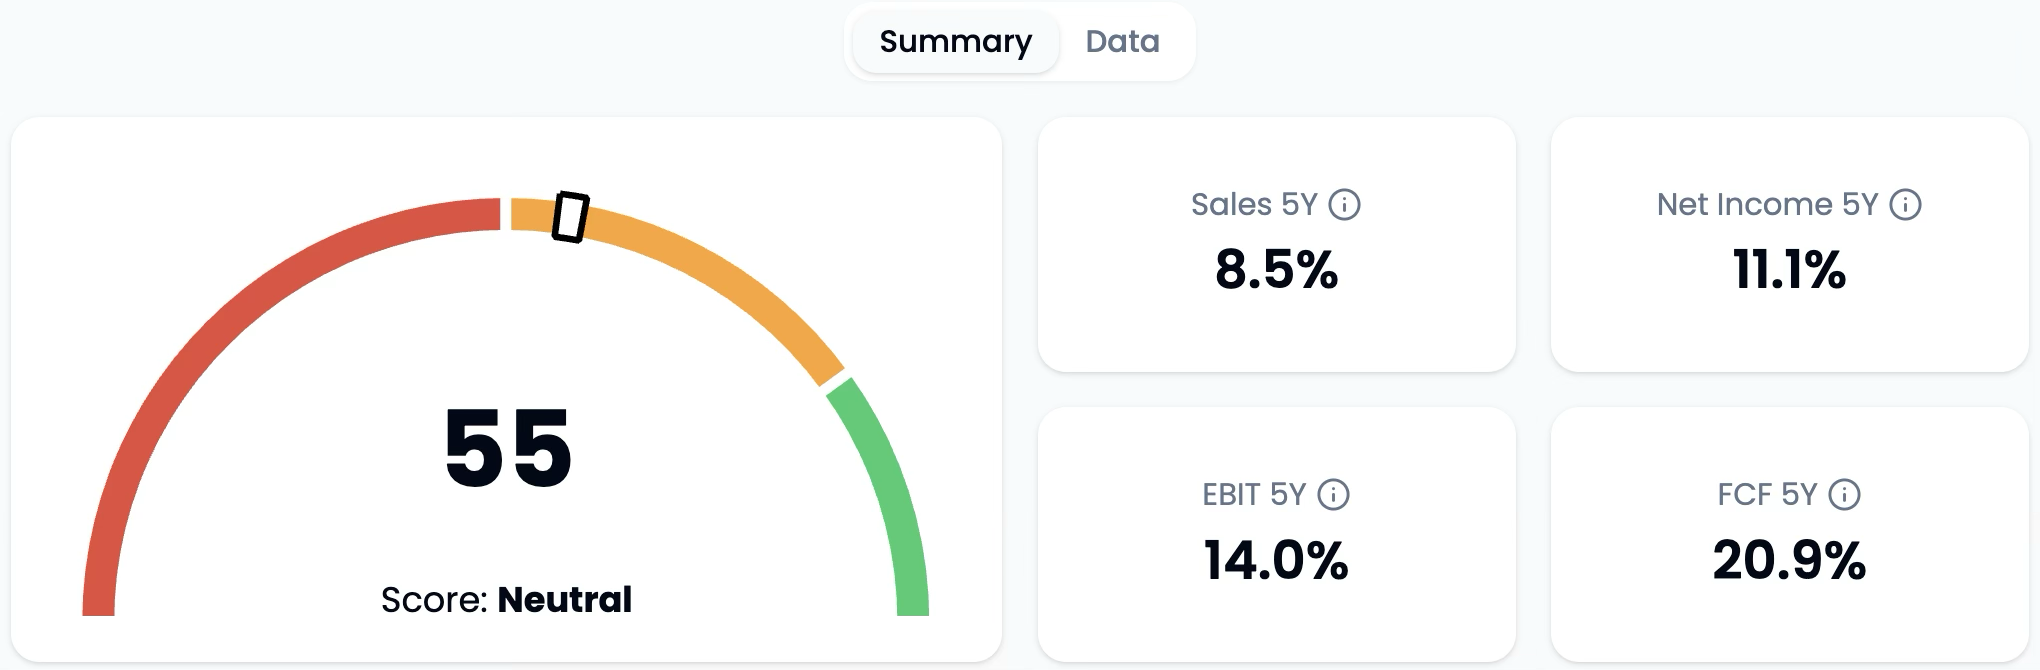
\includegraphics[width=0.8\textwidth]{images/tweenvest/value score.png}
    \caption{Tweenvest's Value Score}
    \label{fig:valuation_score}
\end{figure}


\subsection{Dividend}
\noindent When analyzing Tweenvest most common investors profile, we see a high tendency to dividend investment.

\vspace{0.5cm}
\noindent The Dividend Score measures the attractiveness, reliability, and growth potential of a company's dividend payments. It helps investors assess whether the dividend is both rewarding today and sustainable for tomorrow—a key concern for many users of the platform that are income-focused and long-term investors using mainly dividends as their principal concern. And it is built from three primary components:

\subsubsection{Safety}
\begin{itemize}
    \item \textbf{Payout Ratio EPS} (DPS / Diluted EPS): Shows if dividends are covered by accounting earnings
    \item \textbf{Payout Ratio FCF} (DPS / Free Cash Flow per Share): Shows if dividends are funded by real cash generation
    \item \textbf{Payout Ratio Owner Earnings} (DPS / Owner Earnings per Share): A conservative test of sustainability (excludes CAPEX)
\end{itemize}

\subsubsection{Growth}
\noindent Measures how consistently and strongly the dividend has grown over time.
\begin{itemize}
    \item \textbf{Ordinary DPS CAGR}: 3-Year, 5-Year, 10-Year growth rates
\end{itemize}

\subsubsection{Yield}
\noindent This evaluates the attractiveness of the dividend today relative to the company's historical averages and sector benchmarks.
\begin{itemize}
    \item \textbf{Dividend Yield} (DPS / Price per Share): Represents how much income an investor receives annually from dividends
\end{itemize}

\vspace{0.5cm}
\noindent These components are individually scored weighted and interpolated against industry benchmarks to form a composite score. Finally, the algorithm adjusts this score based on how many years the dividend has been maintained or increased, rewarding consistency.

\begin{figure}[H]
    \centering
    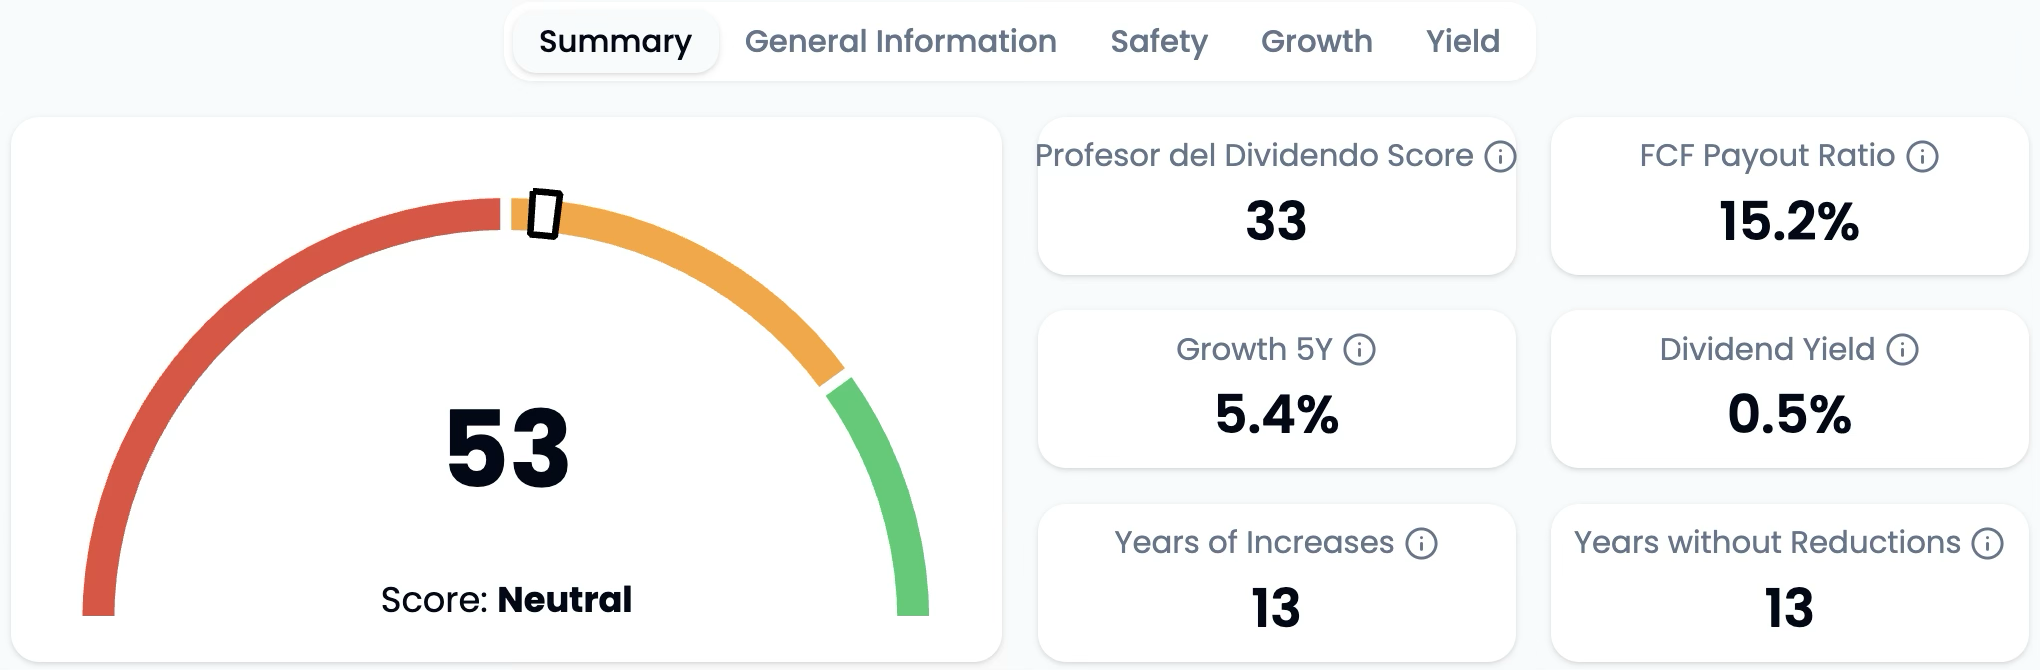
\includegraphics[width=0.8\textwidth]{images/tweenvest/dividend score.png}
    \caption{Tweenvest's Dividend Score}
    \label{fig:dividend_score}
\end{figure}


\section{Problems with the current approach}

\noindent In the context of this thesis, we have to explain the need to make a systematic review of the scores to check wether the simplifications and hypotheses assumed by the financial consensus truly show a company’s ability to create \textit{alpha} over time or not.


\subsection{Unquantified Variables}
\noindent Since the current model only includes variables found in a company's financial statements, there is a significant amount of relevant information being left out, for example:

\begin{itemize}
    \item The \textbf{perceived differentiation of a product} is one such element that may not be properly captured by traditional financial analysis. A trusted brand or strong reputation can allow a company to charge premium prices and build customer loyalty, generating extraordinary long-term profits. For instance, brands like Tiffany or Rolex have high perceived value that justifies elevated prices—something that cannot be easily quantified using standard financial metrics such as profit margins or return on capital.

    \item Additionally, strategies such as \textbf{cost leadership} and offering products at lower prices can provide a significant competitive advantage that is not always directly reflected in financial data.

    \item Companies may also establish \textbf{barriers to entry} and \textbf{high switching costs} for customers, making it more difficult for them to move to competitors. These strategies may involve investments in technology, patents, or simply building long-term customer and employees relationships.
\end{itemize}

\noindent To properly measure these variables, a more exhaustive analysis of each company would be required, pulling from multiple secondary information sources such as news articles, conference transcripts, customer blogs, competitive product reviews, and more. This task is far more difficult to automate via code, as it would require multimodal AI techniques—thus, it will fall outside the scope of this work.

\subsection{Emergent Effects in Complex Systems}

\noindent In complex systems like financial markets, network effects emerge, making most relations between variables not be linear or stationary, adding noise to actual reliable data behind it:

\begin{itemize}
    \item \textbf{Herd behavior} is a network effect where investors tend to follow the actions of others rather than rely on their own analysis. This can amplify market movements, both upward and downward. Herd behavior can lead to speculative bubbles and abrupt corrections when collective expectations shift.

    \item \textbf{Feedback loops} are another network effect where market participants’ actions reinforce existing market behavior. For example, rising asset prices may attract more investors, which in turn drives prices even higher. This type of positive feedback can cause price escalation that becomes detached from underlying fundamentals. Conversely, negative feedback can occur during a sell-off, where falling prices trigger more selling, further accelerating the decline.
    \item \textbf{Macro-level influences} are another crucial factor where broader structural changes—such as political decisions, economic policies, technological shifts, or industry-wide trends—can significantly impact market behavior. These larger forces often operate beyond the scope of individual company analysis and can create ripple effects throughout the entire market ecosystem.
\end{itemize}

\subsection{Linearity and Stationarity}

\subsubsection{Non-linearity}
\noindent The relationships between financial variables are often non-linear, meaning that changes in one variable may not result in proportional changes in another. For example:

\begin{itemize}
    \item \textbf{Economies of scale} can create non-linear relationships between production volume and costs. As a company grows, it may experience decreasing marginal costs due to better resource utilization, bulk purchasing discounts, or spreading fixed costs over larger output.
    
    \item \textbf{Market saturation} can lead to diminishing returns on marketing spend or R\&D investments. Initial investments might yield significant returns, but as the market becomes saturated, additional spending may produce smaller incremental benefits.
    
    \item \textbf{Competitive dynamics} can create threshold effects where small changes in market share or pricing can trigger significant shifts in competitive position or profitability.
\end{itemize}

\subsubsection{Trends}

\noindent Traditionally, standard growth ratios have been used, based on the assumption that in competitive markets, when a new business model or opportunity emerges with above-average margins, entrepreneurs quickly move in to capitalize on it—eventually saturating the opportunity and driving margins back down to average levels over time. But what happens when there is a significant shift in trend? 

\vspace{0.5cm}
\noindent Markets are "fluctuating entities", so static metrics can become problematic when underlying trends change. A clear example is the rise of artificial intelligence and the surge in stock prices of companies involved in the production and development of the necessary technologies.



% ############################### OBJECTIVES #######################
\chapter{Objectives}

\noindent The main objective of this thesis is to check if the scores actually represent an objective and accurate view of the company's ability to generate \textit{alpha} for different time frames, and propose changes to the current algorithm if needed. To do this, we need to follow multiple steps:

\begin{enumerate}
  \item \textbf{System Architecture Enhancement}: Modify Tweenvest's database architecture to enable historical score storage and retrieval and create the datasets for the analysis.
  \item \textbf{Data Curation}: Clean and preprocess the collected data to ensure consistency and reliability, handling missing values and outliers appropriately.
  \item \textbf{Exploratory Analysis}: Process and analyze the data to check if the distributions and correlations between variables, looking for early on patterns to later compare and use for the modeling.
  \item \textbf{Predictive Modeling}: Develop a multiple predictive models to check what is the best way to use the scores for multiple investment strategies.
  \item \textbf{Validation \& Benchmarking}: Back-test the algorithms to check their performance and compare them with S\&P 500 profitabilities.
\end{enumerate}


% ############################### METHODOLOGY #######################
\chapter{Methodology \& Theoretical Framework}

\section{Architecture and Database}
\subsection{Code practices}
Since the code that needs to be changed is used daily in a production environment by Tweenvest, it is important to follow some practices to ensure the code is easy to understand, maintain, and to avoid introducing new bugs.

\begin{itemize}
  \item \textbf{Understanding the code}: Before starting to work on the code, it is important to understand the codebase and the purpose of the code. For this, it is recommended to use some tools like flux diagrams, code comments, and documentation. As it will be shown later on.
  \item \textbf{Testing}: Every function and class should have unit tests that cover all possible scenarios for not introducing new bugs.
  \item \textbf{Logging}: After each feature is implemented, it is important to analyze the logs to check if the feature is working as expected, and to see if there are any possible optimizations to be made in the queries to improve the performance.
  \item \textbf{Code review}: Whenever all of this is done, the code needs to be reviewed and approved by the team to be merged into the main branch.
\end{itemize}

\subsection{Data creation}

%TODO

\subsection{Data storage}

%TODO

\section{Preprocessing}

%TODO

Once we have our final dataset, we need to inspect it and make sure it is consistent and ready to be used for the modeling.

% \vspace{0.5cm}
% \noindent As we will explain later on, many of the models follow the premises of normal distribution.

\subsection{Outlier Detection}

As the models were being trained with raw data, we saw the need to implement some outlier detection to avoid the models to be trained with data that is not representative of the real world.

\subsubsection{Inter Quartile Range}

Just by using the IQR simple method, we saw a significant improvement in the models. Since there are extreme cases that were creating biases in the models.

\subsubsection{Isolation Forest}

Since we know that the data is not normally distributed, and there are representative non-linear relationships between the proffits. We decided to use random forests to detect the outliers.

This method consists in:

% Here we will use some paraphrasing from the original paper

\subsubsection{Single Vector Machine}

After looking at many studies in finance, we decided to also use the Single Vector Machine to detect the outliers.

This method consists in:

% Here we will use some paraphrasing from the original paper

\subsubsection{Local Outlier Factor}

For a more fitted method, we also used the Local Outlier Factor to detect the outliers.

This method consists in:

% Here we will use some paraphrasing from the original paper

\subsubsection{Multimodal Outlier Detection}

There is a big controversy in the field about the best method to detect the outliers, thats why I decided to create a multi-modal method to detect the outliers that combines the results of the different methods.

\vspace{0.5cm}
\noindent This method consists in only deleting the common outliers between the different methods, assuring that the data excluded is only formed by \textit{true outliers}.

% ############################### PREPROCESSING #######################
\subsection{Data Transformation}

To ensure a robust and well-performing model, it is often necessary to preprocess the data by transforming it into a format more suitable for learning algorithms—while preserving the ability to revert it back to its original scale if needed. In many practical cases, rather than analyzing the precise distribution of each variable, we simply standardize the data by centering each feature (subtracting the mean) and scaling it (dividing by the standard deviation), provided the feature is not constant.

\vspace{0.5cm}
\noindent This step is particularly important because many components of machine learning models—such as the RBF kernel in Support Vector Machines or the regularization terms (L1 and L2) in linear models—implicitly assume that features are centered around zero and have comparable variances. Without this adjustment, features with significantly larger variances could dominate the optimization process, leading the model to underweight or ignore more informative but lower-variance features.

\subsubsection{Stansdar Scale}
When trainning the neural networks, it is really important to standardize the data. We can easily use the StandardScaler from the scikit-learn library that uses the transformation of a feature \(x_i\) is calculated as:

\begin{equation}
z_i = \frac{x_i - \mu}{\sigma}
\end{equation}

\noindent where \(\mu\) is the mean of the feature and \(\sigma\) is its standard deviation. This transformation results in a distribution with a mean of 0 and a standard deviation of 1.



\subsubsection{Gaussian Transformation}

In numerous modeling applications, having normally distributed features is advantageous. Power transformations represent a set of parametric, monotonic functions that are an extension of the Box-Cox transformation, designed to convert data from various distributions into approximately Gaussian distributions, thereby reducing variance fluctuations and decreasing distribution asymmetry. These family of transformations are also reversible, so we can easily transform the data back to its original space when needed.

\vspace{0.5cm}
\noindent We finally decided to use the Yeo-Johnson transformation since it allows for negative values.



\begin{equation}
x_i^{(\lambda)} =
\begin{cases}
\frac{[(x_i + 1)^\lambda - 1]}{\lambda}, & \text{if } x_i \geq 0, \lambda \neq 0 \\
\ln(x_i + 1), & \text{if } x_i \geq 0, \lambda = 0 \\
-\frac{[(-x_i + 1)^{2 - \lambda} - 1]}{2 - \lambda}, & \text{if } x_i < 0, \lambda \neq 2 \\
-\ln(-x_i + 1), & \text{if } x_i < 0, \lambda = 2
\end{cases}
\end{equation}

\noindent Where \(\lambda\) is a power parameter that helps minimize the skewness of the data. And since we have already deleted extreme outliers, the final distribution shouldn't be too distorted.

\vspace{0.5cm}

\noindent Here are some exammples of the transformations for different distributions:

\begin{figure}[H]
    \centering
    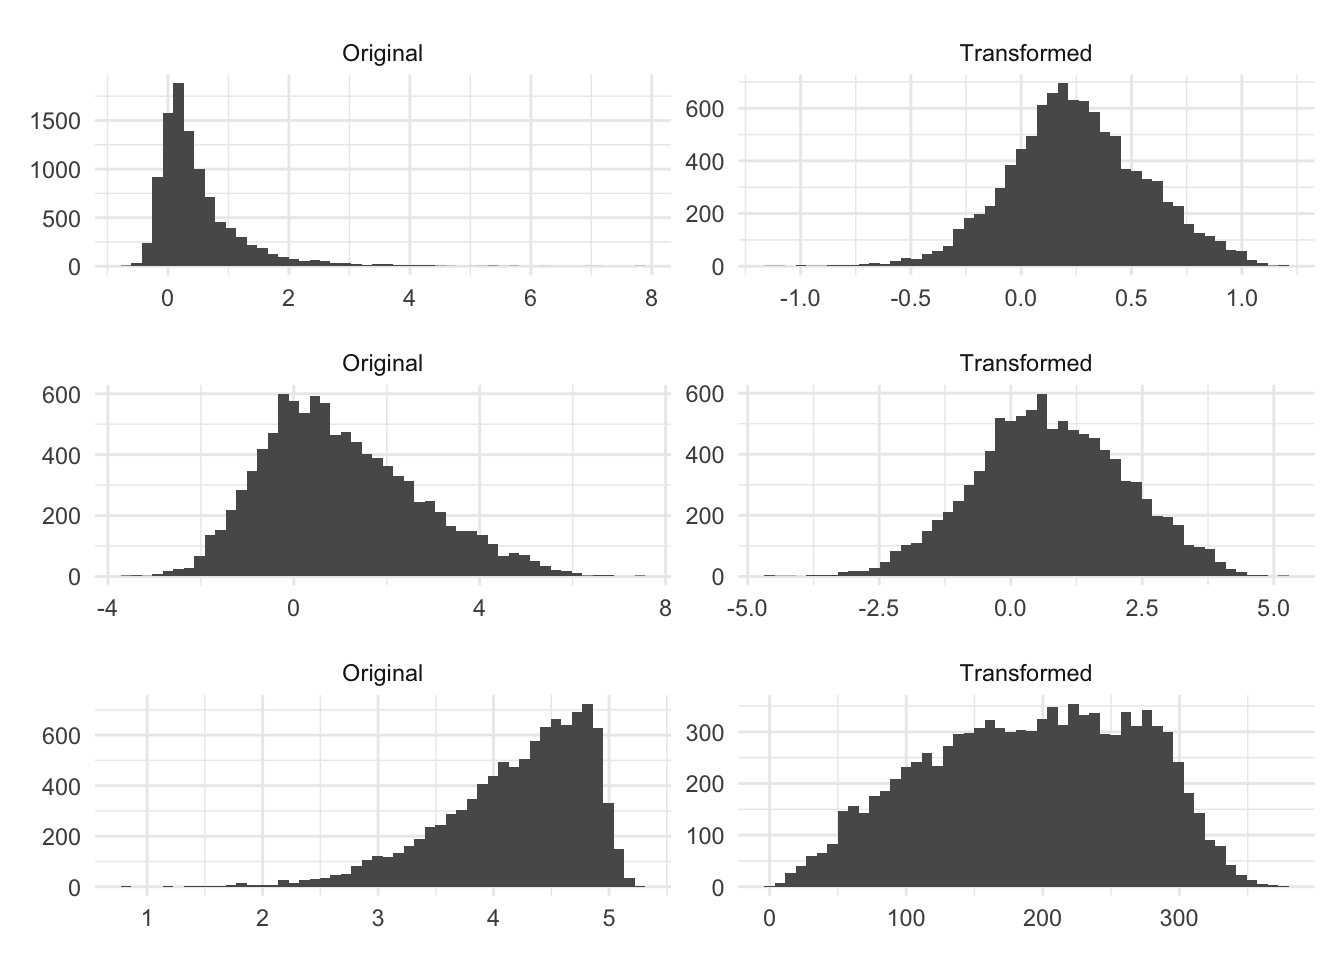
\includegraphics[width=0.8\textwidth]{images/code/transformations/yeo-johnson.png}
    \caption{Yeo-Johnson Transformations examples}
    \label{fig:yeo-johnson}
\end{figure}

% ############################### PREDICTIVE MODELS #######################
\section{Predictive Models}
The main objective of this thesis is to check if the scores have any relation with the future profits of the companies. For doing this in the most generalized way, instead of creating a portfolio following some subjective criteria on the scores, markets and other variables, we will use predictive modeling to check for the actual relationships between the response variables and the predictive ones.

\vspace{0.5cm}
\noindent As a first approach, we will be creating a set of models that separate the scores and the different returns. 

\subsubsection{Response Variables}
We will use different profits that from know one will be representad as \(P_i\) for each time horizon: \(i \in \{1 \text{ month}, 3 \text{ months}, 6 \text{ months}, 1 \text{ year}, 2 \text{ years}, 5 \text{ years}\}\)

\subsubsection{Explanatory Variables}
For being able to train the models, we have different variable categories:

\begin{itemize}
    \item \textbf{Main variables}, these are numerical variables from \textbf{Tweenvest's Scores}, that are in the range of 0 to 100: \(S_j\) where   \(j \in \{\text{ Quality; Value; Dividend; Growth}\}\)
    \item \textbf{Dummy variables}, these are boolean variables that allow us to separate the companies by:
    \begin{itemize}
        \item \textbf{Industry}: \(I_k\) where \(k \in \{\text{Financials; Healthcare; etc.}\}\)
        \item \textbf{Region}: \(R_l\) where \(l \in \{\text{Europe; North America; etc.}\}\)
    \end{itemize}
    \item \textbf{Market Variables}, these are numeric variables that represent the companies \textit{"size"} using the: \textbf{Market Cap} and \textbf{Volume}.
\end{itemize}

\subsection{Regression Models}

To create the econometrical models, we want to be able to understand the actual relationship between the response variables and the explanatory ones. For this we started with the creation of multiple regression models.

\subsubsection{Linear Regression}

As for the first models, we created a series of linear regression models for each factor score that
includes the interactions between the dummy variables and the score used in each model.

\begin{equation}
    \hat{P_i}=\beta_0+\beta_1 \cdot S_j + 
\sum_{n=2}^{N}\beta_{n}\cdot D_n + S_j \cdot \sum_{m=N+1}^{M}\beta_{m}\cdot D_m
\end{equation}

\noindent where:
\begin{itemize}
    \item \(P_i\) is the estimated profit for each time horizon \(i\)
    \item \(S_j\) is the score for each factor \(j\)
    \item \(D_{n,m}\) are the dummy variables for the industry and region, where \(D_{n,m} := I_k \cup R_l\)
    \item \(\beta\) are the coefficients that weight each variable.
\end{itemize}

\noindent For fitting the models, we will also apply a backward selection to remove the variables that are not statistically significant, using the \textbf{p-value} as the criterion.

\subsubsection{Generalized Additive Models}

Because the relationships between the variables are not linear, we also used the Generalized Additive Models (GAM) to check if they are able to capture the non-linear relationships between the variables.

\vspace{0.5cm}
\noindent According to \textcite{pygam2018}, GAMs are smooth semi-parametric models that can capture non-linear relationships between variables. They take the form:

\begin{equation}
    g(\mathbb{E}[y|X]) = \beta_0 + f_1(X_1) + f_2(X_2,X_3) + \dots + f_M(X_N)
\end{equation}

\noindent where:
\begin{itemize}
    \item \(X^T = [X_1, X_2, \dots, X_N]\) are the independent variables
    \item \(y\) is the dependent variable.
    \item \(g()\) is the link function that relates the predictor variables to the expected value of the dependent variable.
    \item \(f_i()\) are feature functions built using penalized B-splines, which automatically model non-linear relationships without requiring manual transformation of variables.
\end{itemize}

\noindent In our case, we will use pyGAMs LinearGAM since it gives a Normal error distribution, and an identity link.

\subsection{Time Series}
In the stock market, the prices of the stocks are not independent of each other, they are correlated in the time series and they also have memory on past behavior of the company. This is what is known as \textbf{Momentum}, so companies that have a good past performance are more likely to have a good future performance, and vice versa.

\vspace{0.5cm}
\noindent For this reason, we contemplated two possibilities:

\subsubsection{ARIMA Models}
To take account the profit tendency, we implemented a ARIMA model to improve the regression models performance by using the residues of the already fitted model:

\begin{equation}
    P_i = \hat{P_i} + {\varepsilon_i} \quad \longleftrightarrow \quad {\varepsilon_i} \sim ARIMA_i(p,d,q)
\end{equation}

\noindent The ARIMA model is defined as:

\begin{equation}
    \phi_i(B_i)(1 - B_i)^{d_i} \varepsilon_i^t = \theta_i(B_i) \eta_i^t
    \end{equation}
    
    \noindent where for each $i$ profit:
    \begin{itemize}
      \item $\varepsilon_i^t$ is the residual at time $t$.
      \item $\eta_i^t$ is a white noise error term (innovation).
      \item $B_i$ is the backshift operator, such that $B \varepsilon_i^t = \varepsilon_i^{t-1}$.
      \item $\phi_i(B) = 1 - \phi_{i1} B - \phi_{i2} B^2 - \dots - \phi_{ip} B^p$ is the autoregressive (AR) polynomial.
      \item $\theta_i(B) = 1 + \theta_{i1} B + \theta_{i2} B^2 + \dots + \theta_{iq} B^q$ is the moving average (MA) polynomial.
      \item $d_i$ is the order of differencing.
    \end{itemize}
    


\subsubsection{Windowed Models}
And for capturing possible memory of the companies behavior in different aspects, we also will implement a windowed model that will use the last \(n\) scores statistical properties to predict future profits.

\vspace{0.5cm}
\noindent So for each score \(j\), we will calculate the average and the standard deviation of the scores over the last \(w\) periods. Let \(S_j^t\) be the score at time \(t\), then for a window of size \(w\):

\begin{equation}
    \bar{S}_j^w = \frac{1}{w} \sum_{i=t-w+1}^{t} S_j^i
\end{equation}

\noindent where:
\begin{itemize}
    \item \(\bar{S}_j^w\) is the average score over window \(w\) for score \(j\)
    \item \(w\) can be 3 or 6 months, 1 or 2 years.
    \item \(t\) is the current time point
    \item \(j\) represents the different scores (Quality, Growth, Value, Dividends)
\end{itemize}

\noindent We will also calculate the standard deviation of the scores over the same window:

\begin{equation}
    \sigma_j^w = \sqrt{\frac{1}{w} \sum_{i=t-w+1}^{t} (S_j^i - \bar{S}_j^w)^2}
\end{equation}

\noindent These statistical measures will be used as additional features in our predictive models to capture the temporal behavior of each score.

\subsection{Neural Networks}

Finally, for trying to capture the non-linear relationships between all the available variables, including the windowed statistical properties, we will use the Neural Networks.



% ############################### DEVELOPMENT AND RESULTS #######################
\chapter{Development and Results}
% Your results

% ############################### DISCUSSION #######################
\chapter{Discussion}
% Analysis and interpretation

% ############################### CONCLUSION #######################
\chapter{Conclusion}
% Summary and conclusions

% ############################### BIBLIOGRAPHY #######################
\printbibliography[heading=bibintoc, title=Bibliography]
\label{sec:biblio}
\newpage

% ############################### APPENDICES #######################
\part{Appendices}
\def\thechapter{\Alph{chapter}}
\makeatletter
\renewcommand{\@chapapp}{Appendix}
\makeatother

\chapter{Additional Listings}
Example appendix content.

\end{document}
